\documentclass[10pt, a4paper]{article}
\usepackage[utf8]{inputenc}
\usepackage{geometry}
\usepackage{amsmath}
\usepackage{amssymb}
\usepackage{amsfonts}
\usepackage{float}
\usepackage{enumerate}
\usepackage{fullpage}
\usepackage{graphicx}
\usepackage{fancyhdr}
\usepackage{siunitx}
\parindent 0ex
\renewcommand{\baselinestretch}{1}

\title{PHY 100 Lab Report}
\author{Irtaza Tanveer Ahmad (24100039@lums.edu.pk) 
\and Muhammad Hamza Sohail (24100100@lums.edu.pk)}
\date{}

\begin{document}
\maketitle

\section*{Helmholtz Resonant Frequency Derivation}
Consider a container of volume $V$ open to the atmosphere through a neck of length $L$ and cross sectional area $A$ as shown in the figure.
\begin{figure}[H]
    \centering
    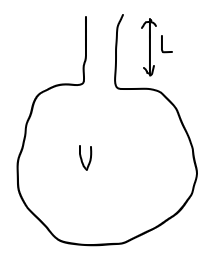
\includegraphics[scale=0.6]{L1.png}
    \label{fig:my_label}
\end{figure}
Let $m$ be the mass of the of the air which occupies the neck of the container. We can then write 
\begin{align}
    m = \rho AL
\end{align}
where $\rho$ is just the density of air. \\
If the column of air present in the neck is pushed down by a small distance $x$, then we can calculate the change in volume of the air in the neck $\Delta V$. This change in volume comes out to be 
\begin{align}
   \Delta V = -Ax
\end{align}
Since $\Delta V$ is negative, this means that the air column is compressed, which means that there is an increase in the pressure acting on that column of air. Let's call this increase in pressure $\Delta P$. \\
Let $k$ represent the coefficient of elasticity of air. This is a constant, and is given by the relation below
\begin{align}
    k = \dfrac{\Delta P}{\dfrac{\Delta V}{V}}
\end{align}
Rearranging yields 
\begin{align}
    \Delta P = \dfrac{k \Delta V}{V}
\end{align}
The mass of air in the column of the container moves down due to the pressure difference $\Delta P$. A difference in pressure corresponds to the action of a force, so we can say that the air column moves down due to some force $F$. 
\begin{align}
    F = A \Delta P
\end{align}
Substituting equations 4 and 2 into equation 5
\begin{align}
        F = \dfrac{k A \Delta V}{V} \\
        F = -\dfrac{A^2 k x}{V}
\end{align}
Notice in the above equation, $F$ is simply a function of the displacement $x$, something we observe when a mass-spring system undergoes simple harmonic motion. However, in order to show that the air column actually undergoes simple harmonic motion, we must obtain an equation of the form 
\begin{align}
    a = -\omega^2 x
\end{align}
In the above equation, $a$ is the acceleration and $\omega$ is the angular frequency which remains constant. \\
Now, another observation to be noted is that the force $F$ which causes the air column to displace a distance $x$ down the neck also causes the air column to undergo an acceleration, which is related by Newton's Second Law
\begin{align}
    F = ma 
\end{align}
Equating equations 9 and 7
\begin{align}
ma = -\dfrac{k A^2 x}{V}
\end{align}
Substituting equation 1 into 10
\begin{align}
    \rho L A a = -\dfrac{k A^2 x}{V} \\
    \rho L a = -\dfrac{k A x}{V} \\
    a = -\dfrac{A k x}{V \rho L} \\
    a = -\left(\dfrac{A k}{V \rho L}\right)x
\end{align}
Since $A$, $k$, $V$, $\rho$ and $L$ are all constants, the column of air does indeed undergo simple harmonic motion. Now we can write 
\begin{align}
    \omega^2 = \dfrac{A k}{V \rho L}
\end{align}
One important observation to be made in the above equation is that the ratio $k/\rho$ is actually the square of the speed of sound (this can easily be seen if we perform a base unit analysis of the quantity $k/\rho$, which yields the units $m^2s^{-2}$). So, if we let $v$ be equal to the speed of sound in air, we can write 
\begin{align}
    \omega^2 = \dfrac{A v^2}{V L}
\end{align}
$\omega$ is related to the Helmholtz frequency $f$ by the relation 
\begin{align}
    \omega = 2 \pi f \\
    \omega^2 = 4 \pi^2 f^2
\end{align}
Plugging equation 18 into 16
\begin{align}
    4 \pi^2 f^2 = \dfrac{A v^2}{V L} \\
    f^2 = \dfrac{v^2}{4 \pi^2} \dfrac{A}{V L} \\
    \boxed{f = \dfrac{v}{2 \pi} \sqrt{\dfrac{A}{V L}}}
\end{align}
Equation 21 is the final expression for the Helmholtz Frequency.

\newpage

\section*{Experimentally Determining the Speed of Sound}
\subsection*{Underlying Idea}
Equation 21 gave us an expression for the Helmholtz Frequency. Performing some manipulation of that expression yields 
\begin{align}
    f^2 = \dfrac{v^2A}{4 \pi^2 L} \dfrac{1}{V}
\end{align}
Equation 22 implies that $f^2$ is directly proportional to $1/V$ (since $v^2$, $A$ and $L$ are constants). So if we plot a graph of $1/V$ on the x-axis and $f^2$ on the y-axis, the graph will ideally be a straight line with a gradient $m$ such that 
\begin{align}
    m = \dfrac{v^2 A}{4 \pi^2 L}
\end{align}
Rearranging Equation 23 
\begin{align}
    v = 2\pi \sqrt{\dfrac{m L}{A}}
\end{align}
From equation 24, it can be easily seen that $L$ and $A$ will contribute towards the overall uncertainty of $v$. 

\subsection*{Experimental Procedure}
\begin{enumerate}
 \item Take a water bottle and fill it with some amount of water. Measure the amount of air in it by subtracting the volume of the water from the maximum capacity of the bottle (which can be measured using a measuring cylinder). This volume is $V$.
 \item Record the length $L$ and cross sectional area $A$ of the bottle’s neck using a ruler. $A$ can be determined by recording the diameter of the bottle’s neck and then using the formula for a circle’s area.
 \item Blow air into the bottle. Use the PhyPhox application to measure the frequency of the sound produced. Repeat the process and measure 3 frequency values $f_1$, $f_2$ and $f_3$ for the same amount of volume. Determine the average frequency $f$ for a specific $V$, as well as $f^2$.
 \item Repeat Step 3 for 5 different values of $V$ for the same water bottle. $V$ can be easily altered by removing water from the bottle. 
 \item Tabulate the following quantities for the water bottle, alongside their overall uncertainties: $V$, $1/V$, $f_1$, $f_2$, $f_3$, $f$ and $f^2$. 
\item Repeat all of the above steps for two additional water bottles.
\item For each bottle, plot a graph of $1/V$ on the x-axis and $f^2$ on the y-axis using MATLAB.
\item Determine the gradient $m$ of the plot for each bottle. Use Equation 24 to determine $v$ for each bottle.
\end{enumerate}

\subsection*{Pre-Experiment Assumptions}
\begin{itemize}
    \item The relationship between $f^2$ and $1/V$ will be directly proportional (i.e. the graph of $f^2$ vs $1/V$ will pass through the origin). 
    \item The PhyPhox Application will be able to accurately record the frequency of the sound despite there being a physical distance between the microphone and the bottle. 
    \item As the volume $V$ increases, $f^2$ should decrease. 
    \item The cross-sectional area $A$ of the bottle is constant throughout the experiment. 
    \item The PhyPhox Application will only measure the frequency of the sound produced due to Helmholtz resonance, and not any other external frequencies. 
\end{itemize}

\subsection*{Experimental Data for Bottle 1}
\begin{table}[H]
\centering
\def\arraystretch{1.6}
\begin{tabular}{|l|l|l|l|l|l|l|}
\hline
$V$ ($10^{-6}$ m^3) & $1/V$ (m^{-3}) & $f_1$ (s^{-1})        & $f_2$ (s^{-1})        & $f_3$ (s^{-1})        & $f$ (s^{-1}) & $f^2$ (s^{-2})   \\ \hline
$750.0 \pm 0.4$                                         & $1300.0 \pm 0.7$                   & $223.80 \pm 0.01$ & $217.70 \pm 0.01$ & $218.70 \pm 0.01$ & $220 \pm 2$ & $48000 \pm 900$ \\ \hline
$900.0 \pm 0.4$                                         & $1100.0 \pm 0.5$                   & $197.10 \pm 0.01$ & $194.70 \pm 0.01$ & $193.90 \pm 0.01$ & $195 \pm 1$ & $38000 \pm 400$ \\ \hline
$1050.0 \pm 0.4$                                        & $952.0 \pm 0.4$                    & $180.10 \pm 0.01$ & $184.20 \pm 0.01$ & $177.40 \pm 0.01$ & $181 \pm 1$ & $32800 \pm 400$ \\ \hline
$1200.0 \pm 0.4$                                        & $830.0 \pm 0.3$                    & $160.70 \pm 0.01$ & $169.3 \pm 0.01$  & $167.5 \pm 0.01$  & $166 \pm 3$ & $27600 \pm 1000$  \\ \hline
$1350.0 \pm 0.4$                                        & $741.0 \pm 0.2$                    & $152.00 \pm 0.01$ & $157.60 \pm 0.01$ & $154.50 \pm 0.01$ & $155 \pm 2$ & $24000 \pm 600$ \\ \hline
\end{tabular}
\caption {Experimental data for Bottle 1, including uncertainties}
\end{table}

\begin{figure}[H]
    \centering
    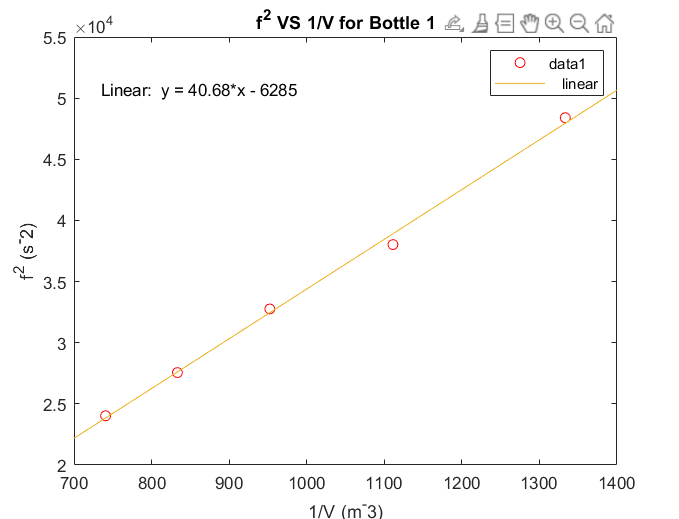
\includegraphics{B1.png}
    \caption{MATLAB Plot for Bottle 1}
\end{figure}

For Bottle 1: 
\begin{itemize}
\item $L = (0.018 \pm 0.001) \si{m}$ 
\item $A = (2.7 \pm 0.8) \times 10^{-4}\si{m^2}$
\item $m = 40.68 \si{s^{-2}m^{3}}$
\end{itemize}
Using Equation 24 to determine the speed of sound for Bottle 1
$$\boxed{v = (337 \pm 50) \si{ms^{-1}}}$$
This value of $v$ has a 4.7\% discrepancy from the true speed of sound ($343 \si{ms^{-1}}$).

\subsection*{Experimental Data for Bottle 2}
\begin{table}[H]
\centering
\def\arraystretch{1.6}
\begin{tabular}{|l|l|l|l|l|l|l|}
\hline
$V$ ($10^{-6}$ m^3) & $1/V$ (m^{-3}) & $f_1$ (s^{-1})        & $f_2$ (s^{-1})        & $f_3$ (s^{-1})        & $f$ (s^{-1}) & $f^2$ (s^{-2})   \\ \hline
$390.0 \pm 0.4$                                         & $2600 \pm 3$                   & $180.80 \pm 0.01$ & $182.80 \pm 0.01$ & $179.40 \pm 0.01$ & $181 \pm 1$ & $32800 \pm 400$\\\hline
$460.0 \pm 0.4$                                         & $2200 \pm 2$                   & $166.30 \pm 0.01$ & $165.10 \pm 0.01$ & $165.70 \pm 0.01$ & $165.7 \pm 0.3$ & $27460 \pm 100$  \\\hline
$530.0 \pm 0.4$                                        & $1900 \pm 1$                    & $154.50 \pm 0.01$ & $158.00 \pm 0.01$ & $159.70 \pm 0.01$ & $157 \pm 2$ & $24600 \pm 600$ \\ \hline
$600.0 \pm 0.4$                                        & $1700 \pm 1$                    & $151.60 \pm 0.01$ & $154.50 \pm 0.01$  & $150.60 \pm 0.01$  & $152 \pm 1$ & $23100 \pm 300$ \\ \hline
$670.0 \pm 0.4$                                        & $1500.0 \pm 0.9$                    & $144.70 \pm 0.01$ & $143.40 \pm 0.01$ & $144.20 \pm 0.01$ & $144.1 \pm 0.4$ & $20760 \pm 100$\\ \hline
\end{tabular}
\caption{Experimental data for Bottle 2, including uncertainties }
\end{table}

\begin{figure}[H]
    \centering
    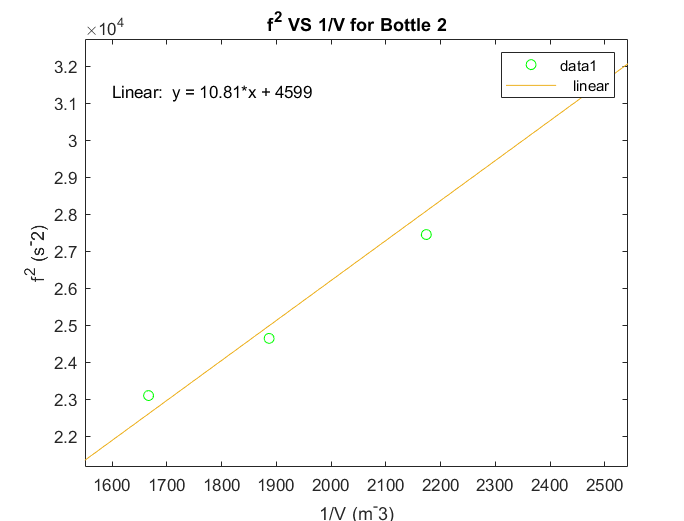
\includegraphics{B2.png}
    \caption{MATLAB Plot for Bottle 2}
\end{figure}

For Bottle 2: 
\begin{itemize}
\item $L = (0.038 \pm 0.001) \si{m}$ 
\item $A = (1.3 \pm 0.4) \times 10^{-4}\si{m^2}$
\item $m = 10.81 \si{s^{-2}m^{3}}$
\end{itemize}
Using Equation 24 to determine the speed of sound for Bottle 2
$$\boxed{v = (353 \pm 50) \si{ms^{-1}}}$$
This value of $v$ has a 2.9\% discrepancy from the true speed of sound ($343 \si{ms^{-1}}$).

\subsection*{Experimental Data for Bottle 3}
\begin{table}[H]
\centering
\def\arraystretch{1.6}
\begin{tabular}{|l|l|l|l|l|l|l|}
\hline
$V$ ($10^{-6}$ m^3) & $1/V$ (m^{-3}) & $f_1$ (s^{-1})        & $f_2$ (s^{-1})        & $f_3$ (s^{-1})        & $f$ (s^{-1}) & $f^2$ (s^{-2})   \\ \hline
$250.0 \pm 0.4$                                         & $4000 \pm 6$                   & $307.00 \pm 0.01$ & $303.20 \pm 0.01$ & $305.00 \pm 0.01$ & $305 \pm 1$ & $93000 \pm 600$ \\\hline
$300.0 \pm 0.4$                                         & $3300 \pm 4$                   & $285.10 \pm 0.01$ & $280.10 \pm 0.01$ & $283.40 \pm 0.01$ & $282 \pm 2$ & $79500 \pm 1000$ \\\hline
$350.0 \pm 0.4$                                        & $2900 \pm 3$                    & $260.30 \pm 0.01$ & $261.70 \pm 0.01$ & $261.70 \pm 0.01$ & $261.2 \pm 0.5$ & $68220 \pm 300$ \\ \hline
$400.0 \pm 0.4$                                        & $2500 \pm 2$                    & $243.10 \pm 0.01$ & $245.60 \pm 0.01$  & $246.90 \pm 0.01$  & $245 \pm 1$ & $60000 \pm 500$ \\ \hline
$450.0 \pm 0.4$                                        & $2200 \pm 2$                    & $229.20 \pm 0.01$ & $228.00 \pm 0.01$ & $230.30 \pm 0.01$ & $229.2 \pm 0.8$ & $52530 \pm 400$ \\ \hline
\end{tabular}
\caption{Experimental Data for Bottle 3, including uncertainties}
\end{table}

\begin{figure}[H]
    \centering
    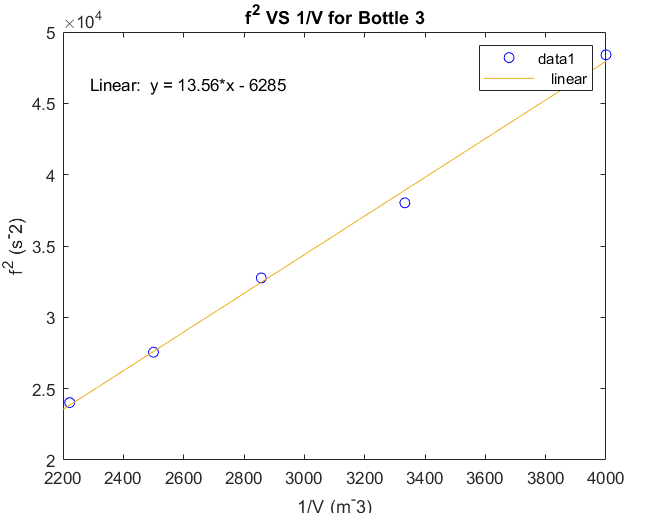
\includegraphics{B3.png}
    \caption{MATLAB Plot for Bottle 3}
\end{figure}

For Bottle 3: 
\begin{itemize}
\item $L = (0.034 \pm 0.001) \si{m}$ 
\item $A = (1.5 \pm 0.7) \times 10^{-4}\si{m^2}$
\item $m = 13.56 \si{s^{-2}m^{3}}$
\end{itemize}
Using Equation 24 to determine the speed of sound for Bottle 3
$$\boxed{v = (348 \pm 80) \si{ms^{-1}}}$$
This value of $v$ has a 1.5\% discrepancy from the true speed of sound ($343 \si{ms^{-1}}$).

\newpage

\section*{Interpretation of Results}
The experimental results certainly do correspond with the theoretical prediction, that as the volume $V$ increases, $f^2$ should decrease. However,in the case of all 3 bottles, none of the graphs for $f^2$ vs $1/V$ did not end up passing through the origin, despite the theoretical prediction that both quantities are directly proportional. This is likely what led to the discrepancies observed in the $v$ values determined for each bottle. Sources of error in the experimental procedure are likely to be the causes for this offset.

\section*{Limitations and Sources of Error}
\begin{itemize}
    \item The use of a measuring cylinder allowed for accurate measurements of the volume of water used in each set of the experimental process, however even these values were not exact due to the presence of a meniscus in the cylinder at the time of measurement which surely led to slight errors in the volume of the water within each bottle and ultimately also propagated itself in measurements of frequency.
    \item Another limitation of the procedure was the low precision of the measurements of frequency as made by the PhyPhox app. This led to a large range of frequencies being possible for any specific volume of water and was a significant source of error in the experiment.
    \item The non-uniformity of the different bottles used was another limitation of the procedure employed. For example, one of the bottles used had ripples, warps, and was made of a softer (more malleable) plastic while another bottle was smooth, sleek and inflexible. These dissimilarities also contributed to the error of the anticipated experimental model.
    \item The measurements of the length and diameter of the bottle spouts were also a part of the experimental data however due to the abnormal shapes of these spouts accurate calculations were somewhat difficult to make especially considering the fact that the mode of measurement (meter rule) was not ideal for this specific purpose. This limitation led to some uncertainty in the measurement of the lengths of these quantities and thus, by definition, the cross sectional area of the spouts, which would act as another potential source of error.  
    \item The cross-sectional area $A$ of the bottle's neck might not remain constant throughout the experiment due to water sticking to sides of the bottle. 
    \item The frequency values measured by the PhyPhox Application could be slightly skewed due to background noise which might have contributed towards the final frequency measurement.
\end{itemize}
\section*{Potential Improvements to the Experimental Procedure}
\begin{itemize}
    \item A larger number of measurements of frequency could be made in for each individual measurement of volume. This would help to more accurately ascertain the true value of the frequency of sound emitted and reduce the error caused by any single erroneous reading.
    \item An alternative improvement to remedy the inaccuracy of measurements in frequency is the use of specialized equipment for this purpose in the form of a decibel meter. Such an instrument would surely produce a more accurate and reliable measure of the frequency of sound produced as compared to a phone application. 
    \item Another possible improvement to the experiment is the use of bottles with comparatively smaller volumes. Such bottles would result in a higher pitched frequency which would be more distinct and easier to distinguish from background noise; something that is considerably harder to do for in the case of the larger volume counterparts.
    \item The use of three or more bottles which are equivalent in their qualities and composition would help to establish uniformity in the experimental procedure and reduce any minor errors caused by such discrepancies.
    \item Making use of a more accurate instrument, such as vernier calipers, in order to measure the length and internal diameter of the spout of each bottle would result in more accurate values of the resonance frequency as calculated by the deduced mathematical model.
    \item Use a blow-dryer to effectively dry all of the water droplets on the bottle so that $A$ remains constant.
    \item Perform the experiment in a quiet environment so that the PhyPhox Application does not register frequencies due to external noises.
\end{itemize}

\section*{Applications of Helmholtz Resonance}
\subsection*{Architectural Acoustics}
Helmholtz resonators can be used as sound absorbing structures in architectural acoustics. In such cases the resonators are designed in a manner such that they have a resonance frequency equivalent to the frequency of sounds which are to be eliminated. Through the process of destructive interference between standing waves, the unwanted sounds are cancelled out. This concept is often used in buildings and theatres in order to eliminate undesirable low frequency sounds.
\begin{figure}[H]
    \centering
    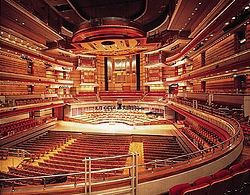
\includegraphics{H1.jpg}
    \caption{Helmholtz resonators are frequently used in architectural acoustics such as within theatres}
\end{figure}
\subsection*{Measuring the Volume of Liquids}
In acoustic theory the value of the resonant frequency can be quantitatively related to the volume of a Helmholtz resonator (as has been previously proven). Thus if the resonance frequency of the resonator is known we can effectively work backwards to find the volume of the chamber and thus the volume of liquid contained within. 
\begin{figure}[H]
    \centering
    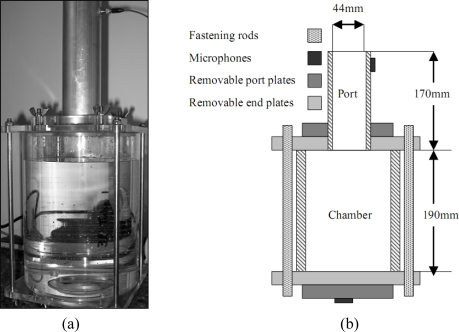
\includegraphics[scale = 4]{H2.png}
    \caption{Depiction of an experimental setup where the volume of chamber is to determined using Helmholtz resonance}
\end{figure}
\subsection*{Rocket Engines}
High frequency combustion instability is a problem which can cause serious damage to the rocket engine. The addition of Helmholtz resonators within the combustion chamber reduces the force of this instability. This is achieved by lining the chamber with dozens of resonators with high resonance frequencies. The resonators dampen the effect of high frequency waves by effectively cancelling them. This reduces unnecessary oscillations within the chamber ultimately leading to a stabilization of the rocket engine.
\begin{figure}[H]
    \centering
    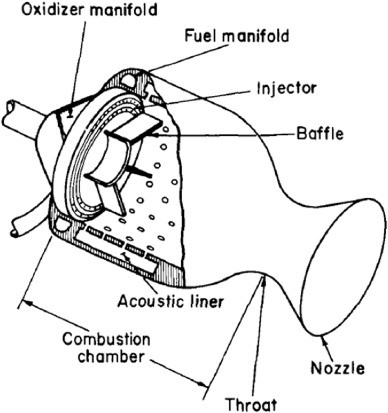
\includegraphics[scale=0.7]{H3.jpg}
    \caption{Cross section of a rocket combustion chamber.  The perforated acoustic lining acts as dozens of Helmholtz resonators}
\end{figure}
\end{document}